\documentclass{article}
\usepackage{amsmath, sfmath, multicol, tkz-euclide, array, enumerate, tcolorbox, tabularray}
\renewcommand{\familydefault}{\sfdefault}
\setlength{\parindent}{0cm}
\pagestyle{empty}
\usepackage[left=1in, top=0.5in, right=1in, bottom=0.5in]{geometry}
\tikzset{>=stealth}
\tcbset{colback=white}

\newcounter{example}[section]
\newenvironment{example}[1][]{\refstepcounter{example}\par\medskip
   {\color{red}\textbf{Example~\theexample. #1}}}{\medskip}

\begin{document}

\section*{Similarity Transformations}

\begin{tcolorbox}[colframe=orange!70!white, coltitle=black, title=\textbf{Today I Can}]
\begin{enumerate}
    \item Identify similarity transformations and verify properties of similarity.
\end{enumerate}
\end{tcolorbox}
\bigskip 

\begin{example}
$\triangle DEF$ has vertices $D(2,0), \, E(1,4), \, \text{ and } F(4,2)$. What is the image of $\triangle DEF$ when you apply each composition?
\begin{multicols}{2}
\begin{enumerate}[(a)]
    \item $D_{1.5} \circ R_{y\text{-axis}}$
    \item $R_{y\text{-axis}} \circ D_{1.5}$
\end{enumerate}
\end{multicols}
\begin{minipage}{0.5\textwidth}
    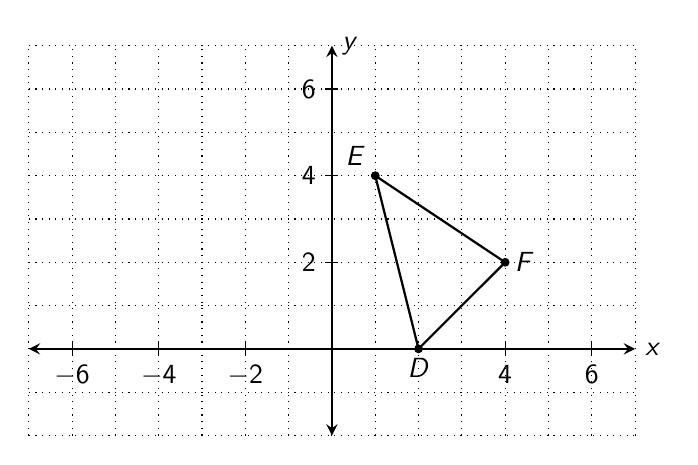
\begin{tikzpicture}[scale=0.55]
    \draw[dotted] (-7,-2) grid (7,7);
    \draw[<->, thick] (-7,0) -- (7,0) node [right] {$x$};
    \draw[<->, thick] (0,-2) -- (0,7) node [right] {$y$};
    \foreach \x in {-6,-4,-2,4,6}
    \draw (\x, 0.15) -- (\x, -0.15) node [below] {$\x$};
    \foreach \y in {2,4,6}
    \draw (0.15, \y) -- (-0.15, \y) node [left] {$\y$};
    \coordinate (D) at (2,0);
    \coordinate (E) at (1,4);
    \coordinate (F) at (4,2);
    \draw[thick] (D) -- (E) -- (F) -- cycle;
    \draw[fill=black] (D) circle [radius = 2.5pt] node [below] {$D$};
    \draw[fill=black] (E) circle [radius = 2.5pt] node [above left] {$E$};
    \draw[fill=black] (F) circle [radius = 2.5pt] node [right] {$F$};
    \end{tikzpicture}
\end{minipage}
\begin{minipage}{0.45\textwidth}
    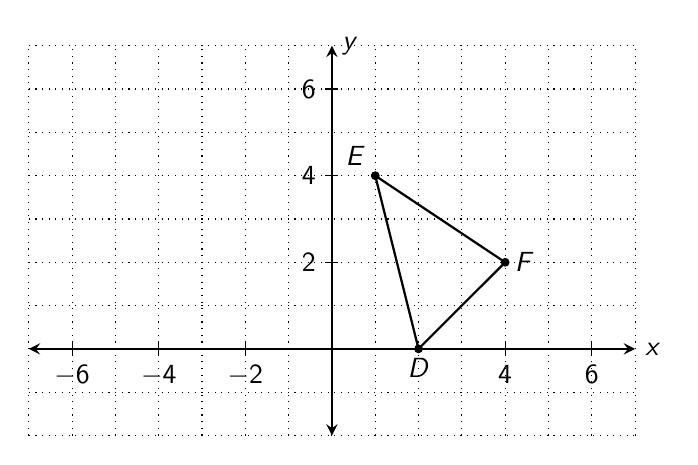
\begin{tikzpicture}[scale=0.55]
    \draw[dotted] (-7,-2) grid (7,7);
    \draw[<->, thick] (-7,0) -- (7,0) node [right] {$x$};
    \draw[<->, thick] (0,-2) -- (0,7) node [right] {$y$};
    \foreach \x in {-6,-4,-2,4,6}
    \draw (\x, 0.15) -- (\x, -0.15) node [below] {$\x$};
    \foreach \y in {2,4,6}
    \draw (0.15, \y) -- (-0.15, \y) node [left] {$\y$};
    \coordinate (D) at (2,0);
    \coordinate (E) at (1,4);
    \coordinate (F) at (4,2);
    \draw[thick] (D) -- (E) -- (F) -- cycle;
    \draw[fill=black] (D) circle [radius = 2.5pt] node [below] {$D$};
    \draw[fill=black] (E) circle [radius = 2.5pt] node [above left] {$E$};
    \draw[fill=black] (F) circle [radius = 2.5pt] node [right] {$F$};
    \end{tikzpicture}
\end{minipage}
\end{example}

\vfill 
\newpage 

\begin{example}
What is a composition of rigid motions and dilations that maps each of the following?
\begin{multicols}{2}
    \begin{enumerate}[(a)]
        \item $\triangle RST$ to $\triangle PYZ$
        \item $ABCD$ to $MNHP$
    \end{enumerate}
\end{multicols}
\begin{minipage}{0.5\textwidth}
    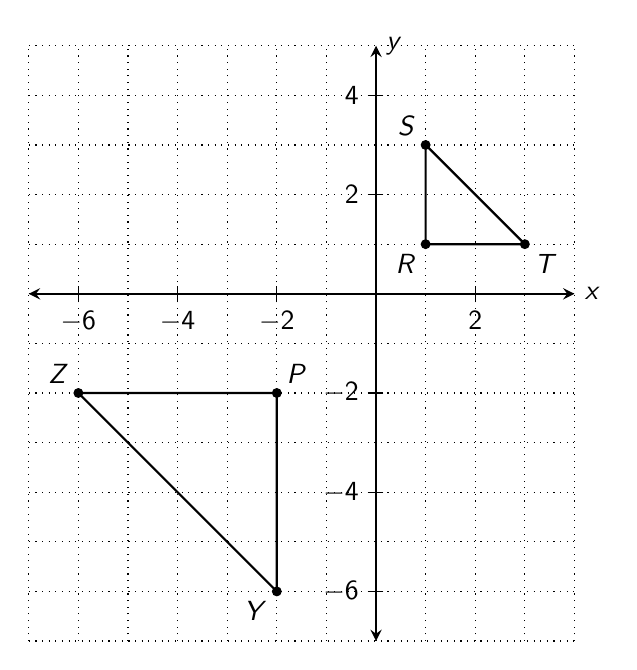
\begin{tikzpicture}[scale=0.63]
    \draw[dotted] (-7,-7) grid (4,5);
    \draw[<->, thick] (-7,0) -- (4,0) node [right] {$x$};
    \draw[<->, thick] (0,-7) -- (0,5) node [right] {$y$};
    \foreach \x in {-6,-4,-2,2}
    \draw (\x, 0.15) -- (\x, -0.15) node [below] {$\x$};
    \foreach \y in {-6,-4,-2,2,4}
    \draw (0.15, \y) -- (-0.15, \y) node [left] {$\y$};
    \coordinate (R) at (1,1);
    \coordinate (S) at (1,3);
    \coordinate (T) at (3,1);
    \draw[thick] (R) -- (S) -- (T) -- cycle;
    \draw[fill=black] (R) circle [radius = 2.5pt] node [below left] {$R$};
    \draw[fill=black] (S) circle [radius = 2.5pt] node [above left] {$S$};
    \draw[fill=black] (T) circle [radius = 2.5pt] node [below right] {$T$};
    \coordinate (P) at (-2,-2);
    \coordinate (Y) at (-2,-6);
    \coordinate (Z) at (-6,-2);
    \draw[thick] (P) -- (Y) -- (Z) -- cycle;
    \draw[fill=black] (P) circle [radius = 2.5pt] node [above right] {$P$};
    \draw[fill=black] (Y) circle [radius = 2.5pt] node [below left] {$Y$};
    \draw[fill=black] (Z) circle [radius = 2.5pt] node [above left] {$Z$};
    \end{tikzpicture}    
\end{minipage}
\begin{minipage}{0.5\textwidth}
    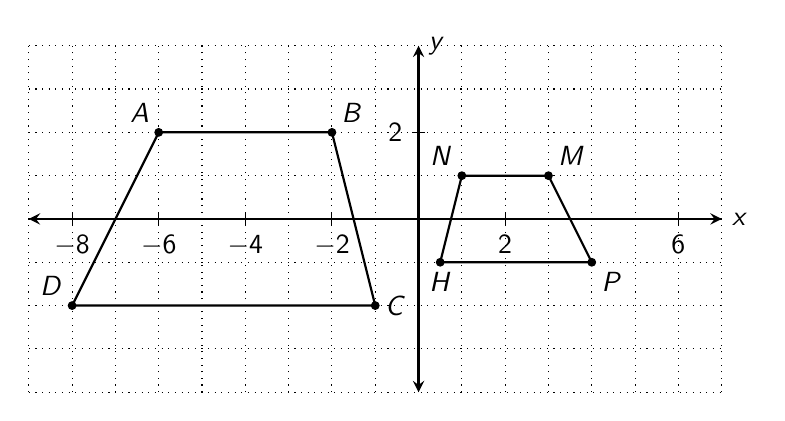
\begin{tikzpicture}[scale=0.55]
    \draw[dotted] (-9,-4) grid (7,4);
    \draw[<->, thick] (-9,0) -- (7,0) node [right] {$x$};
    \draw[<->, thick] (0,-4) -- (0,4) node [right] {$y$};
    \foreach \x in {-8,-6,-4,-2,2,6}
    \draw (\x, 0.15) -- (\x, -0.15) node [below] {$\x$};
    \foreach \y in {2}
    \draw (0.15, \y) -- (-0.15, \y) node [left] {$\y$};    
    \coordinate (A) at (-6,2);
    \coordinate (B) at (-2,2);
    \coordinate (C) at (-1,-2);
    \coordinate (D) at (-8,-2);
    \draw[thick] (A) -- (B) -- (C) -- (D) -- cycle;
    \coordinate (M) at (3,1);
    \coordinate (N) at (1,1);
    \coordinate (H) at (0.5,-1);
    \coordinate (P) at (4,-1);
    \draw[thick] (M) -- (N) -- (H) -- (P) -- cycle;
    \draw[fill=black] (A) circle [radius = 2.5pt] node [above left] {$A$};
    \draw[fill=black] (B) circle [radius = 2.5pt] node [above right] {$B$};
    \draw[fill=black] (C) circle [radius = 2.5pt] node [right] {$C$};
    \draw[fill=black] (D) circle [radius = 2.5pt] node [above left] {$D$};
    \draw[fill=black] (M) circle [radius = 2.5pt] node [above right] {$M$};
    \draw[fill=black] (N) circle [radius = 2.5pt] node [above left] {$N$};
    \draw[fill=black] (H) circle [radius = 2.5pt] node [below] {$H$};
    \draw[fill=black] (P) circle [radius = 2.5pt] node [below right] {$P$};
    \end{tikzpicture}
\end{minipage}
\end{example}

\vfill 

\begin{tcolorbox}[colframe=black!20!white, opacitybacktitle=0.1, coltitle=black, title=\textbf{Similar Figures}]
Two figures are similar if and only if there is a similarity transformation that maps one figure onto the other.
\end{tcolorbox}
\bigskip 

\begin{example}
Is there a similarity transformation that maps $\triangle JKL$ to $\triangle RST$? If so, identify the similarity transformation and write a similarity statement. If not, explain. \newline 

\begin{tikzpicture}
    \tkzDefPoints{0/0/J, 2/1/K, 3/-0.5/L}
    \tkzDrawPolygon(J,K,L)
    \tkzLabelPoints[left](J)
    \tkzLabelPoints[above](K)
    \tkzLabelPoints[right](L)
    \tkzLabelSegment[pos=0.6](J,K){10}
    \tkzLabelSegment(K,L){12}
    \tkzLabelSegment(L,J){16}
    \tkzDefPoints{3/3/R, 6/2/T, 4/1/S}
    \tkzDrawPolygon(R,S,T)
    \tkzLabelPoints[left](R)
    \tkzLabelPoints[below](S)
    \tkzLabelPoints[right](T)
    \tkzLabelSegment(S,R){12}
    \tkzLabelSegment(T,S){16}
    \tkzLabelSegment(R,T){20}
\end{tikzpicture}
\end{example}

\vspace{0.5in}

\end{document}
